\section{Wednesday for MAT4002}\index{Monday_lecture}
\subsection{Remarks on product space} 
\paragraph{Reviewing}
\begin{itemize}
\item
Product Topology: For topological space $(X,\mathcal{T}_X)$ and $(Y,\mathcal{Y})$, define the basis
\[
\mathcal{B}_{X\times Y}=\{U\times V\mid U\in\mathcal{T}_X,V\in\mathcal{T}_Y\}
\]
and the family of union of subsets in $\mathcal{B}_{X\times Y}$ forms a product topology.
\end{itemize}
\begin{proposition}
a ring torus is homeomorphic to the Cartesian product of two circles, say $S^1\times S^1\cong T$.
\end{proposition}
 \begin{proof}
 Define a mapping $f:[0,2\pi]\times [0,2\pi]\to T$ as
 \[
 f(\theta,\phi)=\begin{pmatrix}
(R+r\cos\theta)\cos\phi,
&
(R+r\cos\theta)\sin\phi,
&
r\sin\theta
\end{pmatrix}
 \]
Define $i:T\to\mathbb{R}^3$, we imply
 \[
 i\circ f:[0,2\pi]\times[0,2\pi]\to\mathbb{R}^3\ \text{is continuous}
 \]
 Therefore we imply $f:[0,2\pi]\times [0,2\pi]\to T$ is continuous. Together with the condition that 
\[
\left\{
\begin{aligned}
f(0,y)&=f(2\pi,y)\\
f(x,0)&=f(x,2\pi)
\end{aligned}
\right.
\]
we imply the function $f:S^1\to S^1\to T$ is continuous.
We can also show it is bijective. We can also show $f^{-1}$ is continuous.
 \end{proof}
 
\begin{proposition}
\begin{enumerate}
\item
Let $X\times Y$ be endowed with product topology. 
The projection mappings defined as
\begin{align*}
p_X:&X\times Y\to X,\ \text{with }p_X(x,y) = x\\
p_Y:&X\times Y\to Y,\ \text{with }p_Y(x,y)=y
\end{align*}
are continuous.
\item
(an equivalent definition for product topology)
The product topology is the \emph{coarest topology} on $X\times Y$ such that $p_X$ and $p_Y$ are both continuous.
\item
(an equivalent definition for product topology)
Let $Z$ be a topological space, then the product topology is the unique topology that the red and the blue line in the diagram commutes:
\begin{figure}[H]
\centering
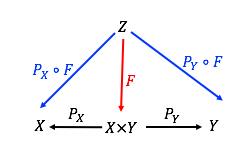
\includegraphics[width=6cm]{week3/p_3}
\caption{Diagram summarizing the statement~(*)}
\end{figure}
namely,
\begin{quotation}
\textit{
the mapping $F:Z\to X\times Y$ is continuous iff both $P_X\circ F:Z\to X$ and $P_Y\circ F:Z\to Y$ are continuous}. (*)
\end{quotation}
\end{enumerate}
\end{proposition}
\begin{proof}
\begin{enumerate}
\item
For any open $U$, we imply $p_X^{-1}(U)=U\times Y\in\mathcal{B}_{X\times Y}\subseteq\mathcal{T}_{X\times Y}$, i.e., $p_X^{-1}(U)$ is open. The same goes for $p_Y$.
\item
It suffices to show any topology $\mathcal{T}$ that meets the condition in (2) must contain $\mathcal{T}_{\text{product}}$. We imply that for $\forall U\in\mathcal{T}_X,V\in\mathcal{T}_Y$, 
\[
\left\{
\begin{aligned}
p_X^{-1}(U)&=U\times X\in\mathcal{T}\\
p_Y^{-1}(V)&=X\times V\in\mathcal{T}
\end{aligned}
\right.
\implies
(U\times Y)\cap(X\times V)=(U\cap X)\times (Y\cap V)=U\times V\in\mathcal{T},
\]
which implies $\mathcal{B}_{X\times Y}\subseteq\mathcal{T}$. Since $\mathcal{T}$ is closed for union operation on subsets, we imply $\mathcal{T}_{\text{product topology}}\subseteq\mathcal{T}$.
\item
\begin{enumerate}
\item
Firstly show that $\mathcal{T}_{\text{product}}$ satisfies (*).
\begin{itemize}
\item
For the forward direction, by (1) we imply both $p_X\circ F$ and $p_Y\circ F$ are continuous, since the composition of continuous functions are continuous as well.
\item
For the reverse direction, for $\forall U\times\mathcal{T}_X,V\in\mathcal{T}_Y$,
\[
F^{-1}(U\times V)=(p_X\circ F)^{-1}(X)\cap (p_Y\circ F)^{-1}(Y),
\]
which is open due to the continuity of $p_X\circ F$ and $p_Y\circ F$.
\end{itemize}
\item
Then we show the uniqueness of $\mathcal{T}_{\text{product}}$. Let $\mathcal{T}$ be another topology $X\times Y$ satisfying (*).
\begin{itemize}
\item
Take $Z=(X\times Y,\mathcal{T})$, and consider the identity mapping $F=\text{id}:Z\to Z$, which is continuous. Therefore $p_X\circ\text{id}$ and $p_Y\circ\text{id}$ are continuous, i.e., $p_X$ and $p_Y$ are continuous. By (2) we imply $\mathcal{T}_{\text{product}}\subseteq\mathcal{T}$.
\item
Take $Z=(X\times Y,\mathcal{T}_{\text{product}})$, and consider the identity mapping $F=\text{id}:Z\to Z$. Note that $p_X\circ F=p_X$ and $p_Y\circ F=p_Y$, which is continuous by (1). Therefore, the identity mapping $F:(X\times Y,\mathcal{T}_{\text{product}})\to(X\times Y,\mathcal{T})$ is continuous, which implies
\[
U=\text{id}^{-1}(U)\subseteq\mathcal{T}_{\text{product}}\ \text{for }\forall U\in\mathcal{T},
\]
i.e., $\mathcal{T}\subseteq\mathcal{T}_{\text{product}}.$
\end{itemize}
The proof is complete.
\end{enumerate}


\end{enumerate}
\end{proof}

\begin{definition}[Disjoint Union]
Let $X\times Y$ be two topological spaces, then the \emph{disjoint union} of $X$ and $Y$ is
\[
X\sqcup Y:=(X\times\{0\})\cup(Y\times\{1\})
\]
\end{definition}
\begin{remark}
\begin{enumerate}
\item
We define that $U$ is open in $X\sqcup Y$ if
\begin{enumerate}
\item
$U\cap(X\times\{0\})$ is open in $X\times\{0\}$; and
\item
$U\cap(Y\times\{1\})$ is open in $Y\times\{1\}$.
\end{enumerate}
We also need to show the weill-definedness for this definition.
\item
$S$ is open in $X\perp Y$ iff $S$ can be expressed as
\[
S=(U\times\{0\})\cup(V\times\{1\})
\]
where $U\subseteq X$ is open and $V\subseteq Y$ is open.
\end{enumerate}
\end{remark}


\subsection{Properties of Topological Spaces}
\subsubsection{Hausdorff Property}
\begin{definition}[First Separation Axiom]
A topological space $X$ satisfies the \emph{first separation axiom} if for any two distinct points $x\ne y\in X$, there exists open $U\ni x$ but not including $y$.
\end{definition}

\begin{proposition}
A topological space $X$ has first separation property if and only if for $\forall x\in X$, $\{x\}$ is closed in $X$.
\end{proposition}
\begin{proof}
\textit{Sufficiency.}
Suppose that $x\ne y$, then construct $U:=X\setminus\{y\}$, which is a open set that contains $x$ but not includes $y$.

\textit{Necessity.}
Take any $x\in X$, then for $\forall y\ne x$, there exists $y\in U_y$ that is open and $x\notin U_y$. Thus 
\[
\{y\}\subseteq U_y\subseteq X\setminus\{x\}
\]
which implies
\[
\bigcup_{y\in X\setminus\{x\}}\{y\}\subseteq
\bigcup_{y\in X\setminus\{x\}}U_y\subseteq
X\setminus\{x\},
\]
i.e., $X\setminus\{x\}=\bigcup_{y\in X\setminus\{x\}}U_y$ is open in $X$, i.e., $\{x\}$ is closed in $X.$
\end{proof}

\begin{definition}[Second separation Axiom]
A topological space satisfies the \emph{second separation axiom} (or $X$ is Hausdorff) if for all $x\ne y$ in $X$, there exists open sets $U,V$ such that
\[
\begin{array}{lll}
x\in U,
&
y\in V,
&
U\cap V=\emptyset
\end{array}
\]
\end{definition}

\begin{example}
All metrizable topological spaces are Hausdorff.

Suppose $d(x,y)=r>0$, then take $B_{r/2}(x)$ and $B_{r/2}(y)$
\end{example}

\begin{example}
Note that a topological space that is \emph{first separable} may not necessarily be \emph{second separable}:

Consider $\mathcal{T}_{\text{co-finite}}$, then $X$ is first separable but not Hausdorff:

Suppose on the contrary that for given $x\ne y$, there exists open sets $U,V$ such that $x\in U,y\in V$, and
\[
U\cap V=\emptyset\implies
X = X\setminus (U\cap V) = (X\setminus U)\cup(X\setminus V),
\]
implying that the union of two finite sets equals $X$, which is infinite, which is a contradiction.
\end{example}

















